\documentclass[border=8pt]{standalone}
\usepackage{amsmath,amssymb}
\usepackage{tikz}
\usetikzlibrary{arrows.meta,calc}
\begin{document}
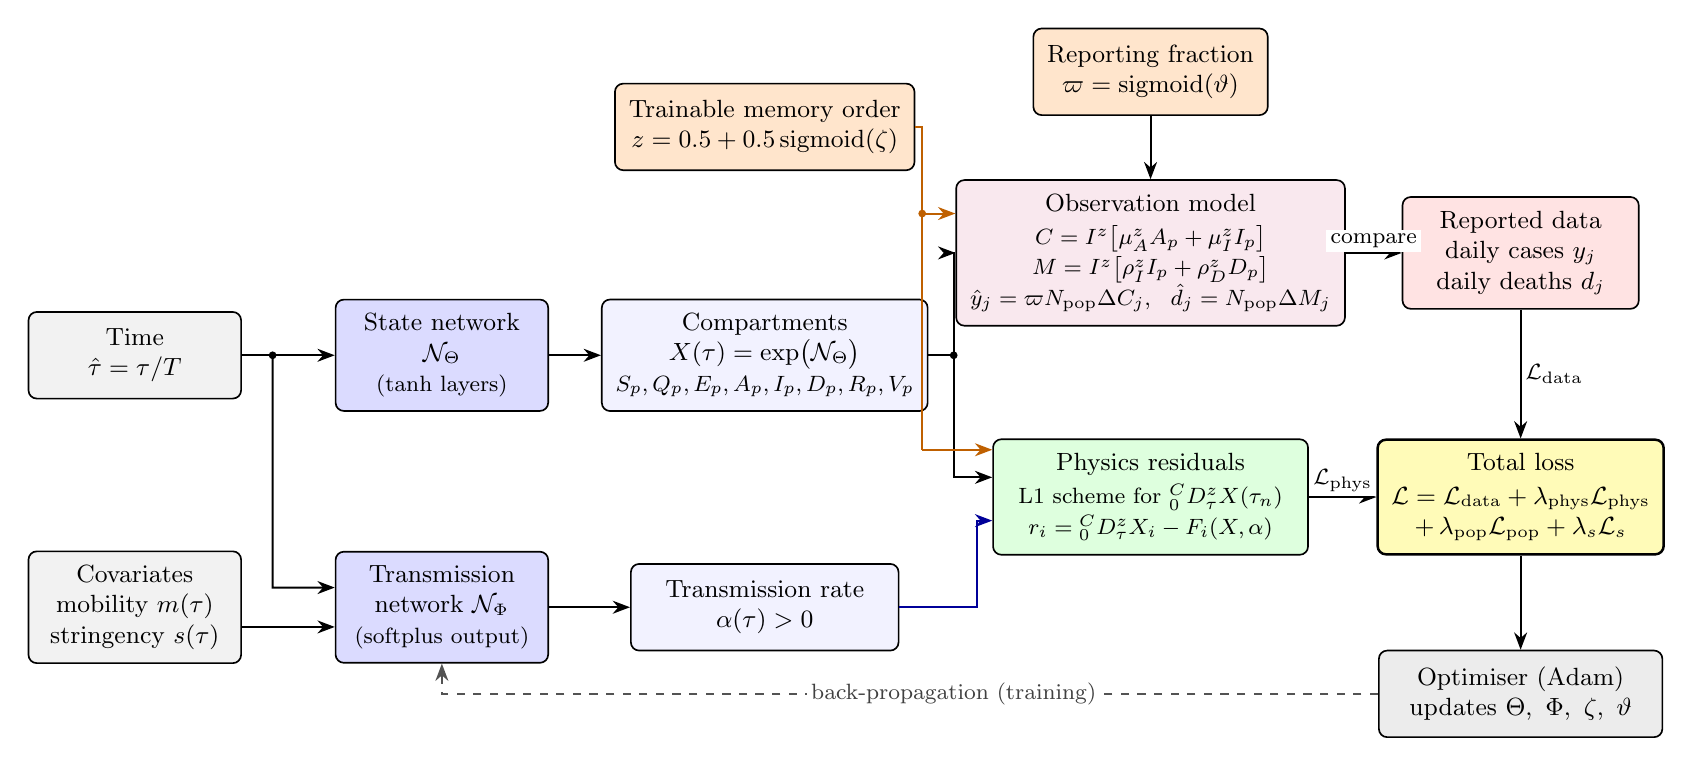
\begin{tikzpicture}[
  font=\small,
  >={Stealth[length=2.2mm]},
  box/.style={draw, rounded corners=3pt, align=center, inner sep=5pt, line width=0.6pt, minimum height=11mm},
  inp/.style={box, fill=gray!10, minimum width=27mm},
  net/.style={box, fill=blue!14, minimum width=27mm},
  outb/.style={box, fill=blue!5, minimum width=34mm},
  par/.style={box, fill=orange!20},
  phys/.style={box, fill=green!13, minimum width=40mm},
  obs/.style={box, fill=purple!9, minimum width=40mm},
  data/.style={box, fill=red!11, minimum width=30mm},
  loss/.style={box, fill=yellow!28, minimum width=36mm, line width=0.9pt},
  arr/.style={->, line width=0.7pt},
  lab/.style={font=\footnotesize, fill=white, inner sep=1.5pt}
]

% ---------------- nodes (fixed grid) ----------------
\node[inp]  (tau)   at (0,0)     {Time\\ $\hat{\tau}=\tau/T$};
\node[inp]  (cov)   at (0,-3.2)  {Covariates\\ mobility $m(\tau)$\\ stringency $s(\tau)$};

\node[net]  (Nth)   at (3.9,0)   {State network\\ $\mathcal{N}_{\Theta}$\\ {\footnotesize (tanh layers)}};
\node[net]  (Nph)   at (3.9,-3.2){Transmission\\ network $\mathcal{N}_{\Phi}$\\ {\footnotesize (softplus output)}};

\node[outb]  (X)     at (8.0,0)   {Compartments\\ $X(\tau)=\exp\!\big(\mathcal{N}_{\Theta}\big)$\\ {\footnotesize $S_p,Q_p,E_p,A_p,I_p,D_p,R_p,V_p$}};
\node[outb]  (alpha) at (8.0,-3.2){Transmission rate\\ $\alpha(\tau)>0$};

\node[par]  (z)     at (8.0,2.9) {Trainable memory order\\ $z=0.5+0.5\,\mathrm{sigmoid}(\zeta)$};
\node[par]  (varpi) at (12.9,3.6){Reporting fraction\\ $\varpi=\mathrm{sigmoid}(\vartheta)$};

\node[obs]  (obs)   at (12.9,1.3){Observation model\\[1pt]
  {\footnotesize $C=I^{z}\big[\mu_A^{z}A_p+\mu_I^{z}I_p\big]$}\\
  {\footnotesize $M=I^{z}\big[\rho_I^{z}I_p+\rho_D^{z}D_p\big]$}\\
  {\footnotesize $\hat y_j=\varpi N_{\mathrm{pop}}\Delta C_j,\ \ \hat d_j=N_{\mathrm{pop}}\Delta M_j$}};
\node[phys] (L1)    at (12.9,-1.8){Physics residuals\\[1pt]
  {\footnotesize L1 scheme for ${}^{C}_{0}D^{z}_{\tau}X(\tau_n)$}\\
  {\footnotesize $r_i={}^{C}_{0}D^{z}_{\tau}X_i-F_i(X,\alpha)$}};

\node[data] (dat)   at (17.6,1.3){Reported data\\ daily cases $y_j$\\ daily deaths $d_j$};
\node[loss] (L)     at (17.6,-1.8){Total loss\\[1pt]
  $\mathcal{L}=\mathcal{L}_{\mathrm{data}}+\lambda_{\mathrm{phys}}\mathcal{L}_{\mathrm{phys}}$\\
  $+\,\lambda_{\mathrm{pop}}\mathcal{L}_{\mathrm{pop}}+\lambda_{s}\mathcal{L}_{s}$};
\node[box, fill=gray!15, minimum width=36mm] (opt) at (17.6,-4.3){Optimiser (Adam)\\ updates $\Theta,\ \Phi,\ \zeta,\ \vartheta$};

% ---------------- arrows ----------------
% inputs -> networks
\draw[arr] (tau) -- (Nth);
\draw[arr] ($(cov.east)+(0,-0.25)$) -- ($(Nph.west)+(0,-0.25)$);
\draw[arr] (1.75,0) -- (1.75,-2.95) -- ($(Nph.west)+(0,0.25)$);
\fill (1.75,0) circle (1.4pt);

% networks -> outputs
\draw[arr] (Nth) -- (X);
\draw[arr] (Nph) -- (alpha);

% compartments -> observation model and physics
\draw[arr] (X.east) -- (10.4,0) |- (obs.west);
\draw[arr] (10.4,0) |- ($(L1.west)+(0,0.25)$);
\fill (10.4,0) circle (1.4pt);

% alpha -> physics
\draw[arr, blue!60!black] (alpha.east) -- (10.7,-3.2) |- ($(L1.west)+(0,-0.3)$);

% z -> observation model and physics
\draw[line width=0.7pt, orange!75!black] (z.east) -- (10.0,2.9) -- (10.0,-1.2);
\draw[arr, orange!75!black] (10.0,1.8) -- ($(obs.west)+(0,0.5)$);
\draw[arr, orange!75!black] (10.0,-1.2) -- ($(L1.west)+(0,0.6)$);
\fill[orange!75!black] (10.0,1.8) circle (1.4pt);

% varpi -> observation model
\draw[arr] (varpi.south) -- (obs.north);

% compare with data
\draw[arr] (obs.east) -- node[lab, above] {compare} (dat.west);

% losses
\draw[arr] (dat.south) -- node[lab, right] {$\mathcal{L}_{\mathrm{data}}$} (L.north);
\draw[arr] (L1.east) -- node[lab, above] {$\mathcal{L}_{\mathrm{phys}}$} (L.west);
\draw[arr] (L) -- (opt);

% back-propagation
\draw[arr, dashed, gray!65!black] (opt.west) -- (3.9,-4.3) -- (Nph.south);
\node[font=\footnotesize, text=gray!50!black, fill=white, inner sep=1.5pt] at (10.4,-4.3) {back-propagation (training)};

\end{tikzpicture}
\end{document}
